%% Section that includes the experiments performed.

This section describes the accomplished experiments that prove how the 
developed system fulfills SKA's requirements for the PPS distribution system. 
\ftglnote{demasiado pretencioso?} The first experiment is a general 
characterization of the PPS distribution system. The second one emulates a 
example of WR network like the one needed to distribute timing in the SKA1-mid, 
and evaluates the synchronization accuracy. Finally, the influence of external 
conditions over the fiber links and its effect on the synchronization accuracy 
is analyzed.

The principal equipment and tools utilized to accomplish the presented 
experiments is depicted below:

\begin{itemize}
    \item Two White Rabbit Switches to emulate a two-hops WR network. Both are 
    hardware version 3.4 and are flashed with the last version of the WR 
    firmware (v5.0).
    
    \item A White Rabbit ZEN Time Provider (WR-ZEN TP) to test the performance 
    of the new developed platform as WR nodes of the SKA facilities. The 
    firmware version is 1.2.
    
    \item A High-resolution counter from Keysight, the 52320A.
    
    \item Multiple components for the setup of the equipment:
    \begin{itemize}
        \item Small form-factor pluggable transceptors (SFPs) to stablish the 
        link between WR devices.
        \item Simplex optical fiber links (G652D). For the device 
        characterization short distance fibers have been used, meanwhile for 
        the scalability and temperature tests we have used long distance links: 
        20 and 50 km respectively.
        \item A OCXO Morion MV89 as frequency reference for the GM mode.
    \end{itemize}
    
\end{itemize}

\subsection{Characterization of the WR-ZEN platform}
\label{subsec: charact_zen}

% Aquí las pruebas típicas de caracterización

The new components included in the clocking's scheme of the WR-ZEN, described in section \ftglnote{Meter ref cuando esté integrado en el resto} 4.1, offer a performance improvement respect to previous WR designs, such as the WRS. 

\missingfigure{Esquema de las medidas realizadas}

The following experiments evaluate phase noise performance of the frequency transfer in WR at different scenarios: a) Grand Master mode, to evaluate how the WR-ZEN syntonizes to an external reference clock. b) Master mode, that reflects the characteristics of the new internal XO of the WR-ZEN. c) Slave mode, to see the behavior of the new design as slave node of the network.

The Free running mode (FR) is not affected by the WR's logic, it is mostly influenced by noise of the crystal oscillator (XO). \textcolor{blue}{TODO: Completar haciendo referencia a la sección de hardware.}

\ftgnote{Las figuras de Phase Noise juntas se ven regular, pero separadas parece que estamos tirando espacio para rellenar...}
\begin{figure}
    \centering
    \begin{subfigure}[t]{0.45\textwidth}
        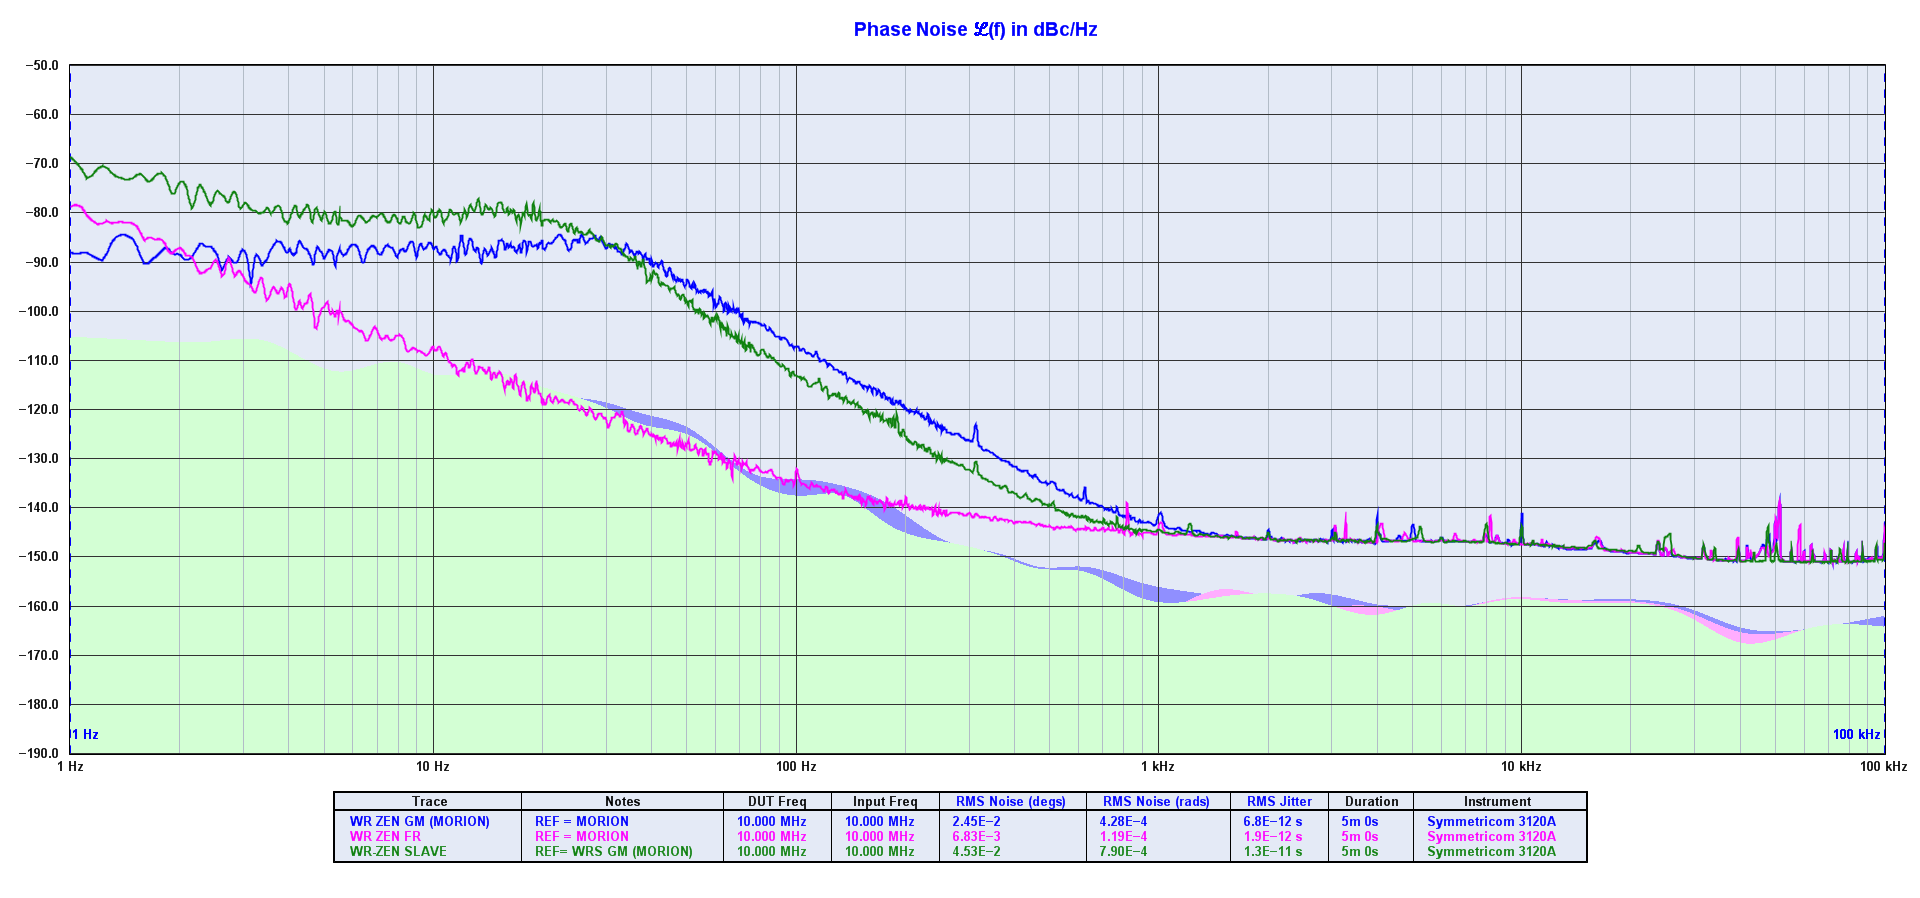
\includegraphics[width=\textwidth]{../measures/img/zen_all}
        \caption[Phase noise plot of the WR-ZEN]{The figure shows the Phase noise plot for the WR-ZEN in the Grand Master, Free Running and Slave modes. Sine wave output is compared to CMOS output.}
        \label{fig:zen_pn_all}
    \end{subfigure}
    ~ % This symbol adds a white space between images
    \begin{subfigure}[t]{0.45\textwidth}
         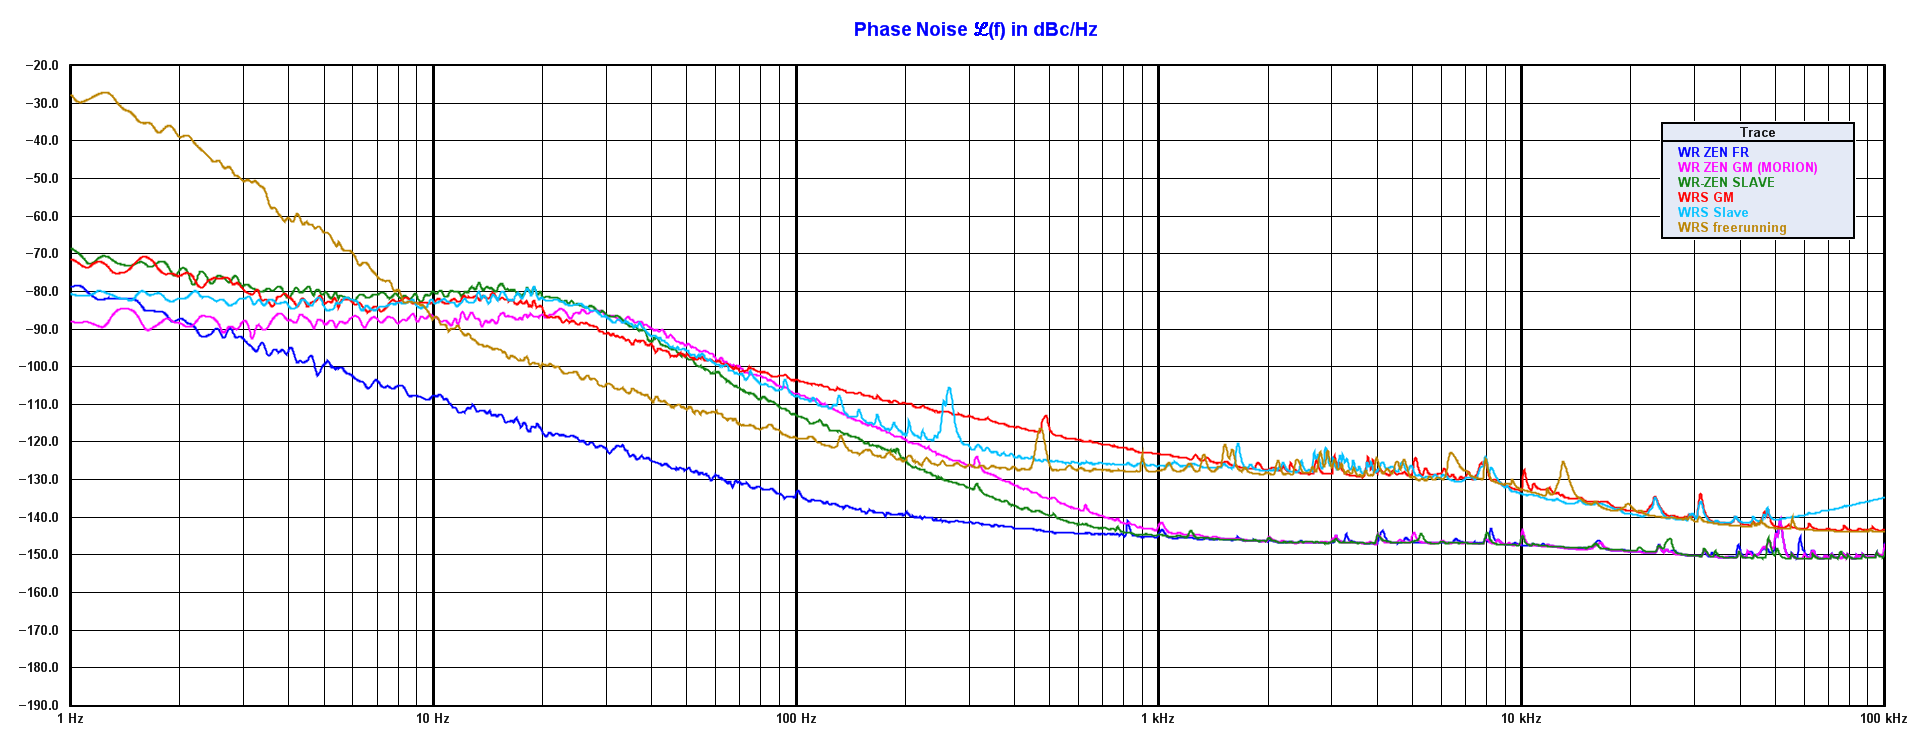
\includegraphics[width=\textwidth]{../measures/img/zen_vs_wrs}
         \caption[Phase noise plot of the WR-ZEN vs WRS]{The figure includes the same phase noise measures for the WRS. In this plot, only the CMOS outputs appear because the WRS doesn't have sine wave output signals.}
         \label{fig:zen_vs_wrs}
    \end{subfigure}
\end{figure}

The following experiments evaluate phase noise performance of the frequency transfer in WR at different scenarios: a) Grand Master mode, to evaluate how the WR-ZEN syntonizes to an external reference clock. b) Master mode, that reflects the characteristics of the new internal XO of the WR-ZEN. c) Slave mode, to see the behavior of the new design as slave node of the network. Different configurations are depicted in fig. ?? to allow the reproduction of the different experiments of this paper.

The Free running mode (FR) is not affected by the WR's logic, it is mostly influenced by noise of the crystal oscillator (XO). A master node is placed at top of a timing network hierarchy, and unlike a Grand Master node, it is not locked to any external reference. So that, a master node with an improved stability will benefit the performance of all the downlink devices connected to it.

It is also relevant to test the performance of the system when locking to an external reference in Grand master mode. Additive noise of the WR-ZEN will be propagated downstream, decreasing the quality of the Grand master's reference clock. It's very important that the system adds low noise in order to not degrade the quality of the external reference clock.

Results included in table \ref{tab:pn_results} ... \textcolor{blue}{TODO: hablar de la frecuencia de corte del softpll y del ddmtd.}
    
\begin{table*}\centering
     \ra{0.8}
     \begin{tabular}{@{} rcccc@{}}%\toprule
         & \multicolumn{4}{c}{\bfseries{RMS jitter (ps)}} \\
         \cmidrule(l){2-5}
         & 1Hz-10Hz & 10Hz-1kHz & 1kHz-100kHz  & 1Hz-100kHz \\ \midrule
         \textbf{Free running}\\
         \small{WRS (CMOS)}             & 62  & 1.7  & 1.1  & 62  \\
         \small{WR-ZEN (\textit{sine})} & 2.1 & 0.24 & 1.4  & 2.5 \\
         \small{WR-ZEN (\textit{CMOS})} & 1.9 & 0.21 & 0.26 & 1.9 \\
         \cmidrule(l){2-5}
         
         \textbf{Grand Master}\\
         \small{WRS (CMOS)}             & 7.3 & 6.7 & 1.1 & 9.9\\
         \small{WR-ZEN (\textit{CMOS})} & 2.8 & 6.2 & 0.26 & 6.8\\
         \cmidrule(l){2-5}
         
         \textbf{Slave node}\\
         \small{WRS (CMOS)}             & 4.9 & 8.2 & 1.2  & 9.7\\
         \small{WR-ZEN (\textit{CMOS})} & 8.5 & 9.3 & 0.24 & 13\\
         
         \bottomrule
        \end{tabular}
        \caption{Phase Noise results extracted from plots in figure \ref{fig:zen_pn_all} and \ref{fig:zen_vs_wrs}.}
        \label{tab:pn_results}
\end{table*}

The slave mode results show that WR-ZEN performs slightly worse than WRS. Noise 
between 1 Hz and 20 Hz increases the RMS Jitter of the WR-ZEN. 
\textcolor{blue}{This may be caused by a poor adjustment of the PI control.}

\subsection{WR scalability for SKA} %% Buscar un nombre mejor
\label{subsec: net_exp}

The next experiment covers a scalability analysis of the WR solution for the 
SKA timing system. In section \ref{sec:ska} there is a estimation of the final 
nodes that need to be synchronized for the SKA1-mid: around 250 endpoints that 
must be synchronized with an accuracy below 5ns. A WR network with only two 
hops is suitable to synchronize up to 306 endnodes by the use of WR Switches as 
Boundary Clocks.

We set up a test network composed by a WRS at the top, which is locked to an 
external time reference, another WRS as intermediate BC and a WR-ZEN as 
endpoint. This configuration allows synchronizing up to 306 WR nodes with an 
expected performance similar to the results obtained in our test for the WR-ZEN.

\begin{figure}
	\centering
	\includegraphics[width=0.7\linewidth]{img/prueba_red}
	\caption[WR Scalability test's setup for SKA]{To evaluate the scalability 
	of the WR solution for the expected SKA1-mid timing network, a sample WR 
	network has been evaluated. At the top there's a WRS as GM, a second layer 
	of WRS to finally provide synchronization to the end-nodes (WR-ZEN).}
	\label{fig:pruebared}
\end{figure}


All the equipment for that test was under laboratory conditions. To connect 
each one of the WR devices we've used a 20km fiber spool and SFPs from 
FiberStore (SFP-GE-BX80 with 1490/1550 nm wavelengths). PPS phase difference is 
measured from the WR-ZEN to the WRS in GM configuration using a Keysight 52320A 
counter along 4 hours.

\begin{figure}
	\centering
	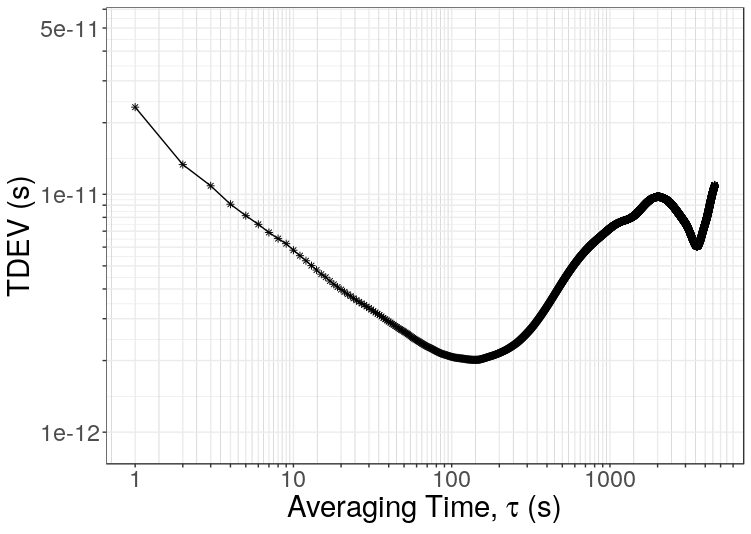
\includegraphics[width=0.9\linewidth]{img/tdev_exp3}
	\caption[TDEV of the end-nodes in the scalability test.]{Time Deviation 
	plot comparing the PPS signal from the end-nodes (WR-ZEN) to the Grand 
	Master of the network.}
	\label{fig:tdevnet}
\end{figure}

TDEV and MTIE values have been calculated by octaves, the numerical values can 
be found in Table \ref{tab:netresults}. Graphical representations are included 
in Figures \ref{fig:tdevnet} and \ref{fig:mtienet} respectively. TDEV results 
show that expected synchronization accuracy for the end-nodes is around tens of 
ps. The maximum PPS error during this test is bounded in hundred of ps, which 
is more than enough what SKA1-mid needs (5ns).

\begin{table*}\centering
	\ra{0.8}
	\begin{tabular}{@{} rcc@{}}%\toprule
		& TDEV (s)  & MTIE (s) \\ \midrule
		\textbf{$\tau$ (s)}\\
		\small{1}     & 2.32509201e-11  & 1.36718750e-10 \\
		\small{2}     & 1.33315382e-11  & 1.36718750e-10 \\
		\small{4}     & 9.08699704e-12  & 1.36718750e-10 \\
		\small{10}    & 5.82194037e-12  & 1.36718750e-10 \\
		\small{20}    & 3.97732795e-12  & 1.36718750e-10 \\
		\small{40}    & 2.91762201e-12  & 1.46484375e-10 \\
		\small{1e2}   & 2.07423753e-12  & 1.46484375e-10 \\
		\small{2e2}   & 2.15075917e-12  & 1.46484375e-10 \\
		\small{4e2}   & 3.37401257e-12  & 1.51367188e-10 \\
		\small{1e3}  & 7.18913143e-12  & 1.66015625e-10 \\
		\small{2e3}  & 9.75471284e-12  & 1.66015625e-10 \\
		\small{4e3}  & 7.54252759e-12  & 1.90429688e-10 \\
		\small{1e4}  &                 & 2.05078125e-10 \\
		
		\bottomrule
	\end{tabular}
	\caption{Results of the scalability analysis.}
	\label{tab:netresults}
\end{table*}

With those results, it's proved that a WR network with two levels can provide 
synchronization to all the equipment expected for the SKA1-mid facilities. 
Although long-distance fiber links have been used for that test, thermal 
influence should be take into account in order to confirm the goodness of the 
WR solution in the SKA timing distribution. The next experiment will evaluate 
how the temperature change in the fiber link can affect the accuracy of the 
synchronization. 


\begin{figure}
	\centering
	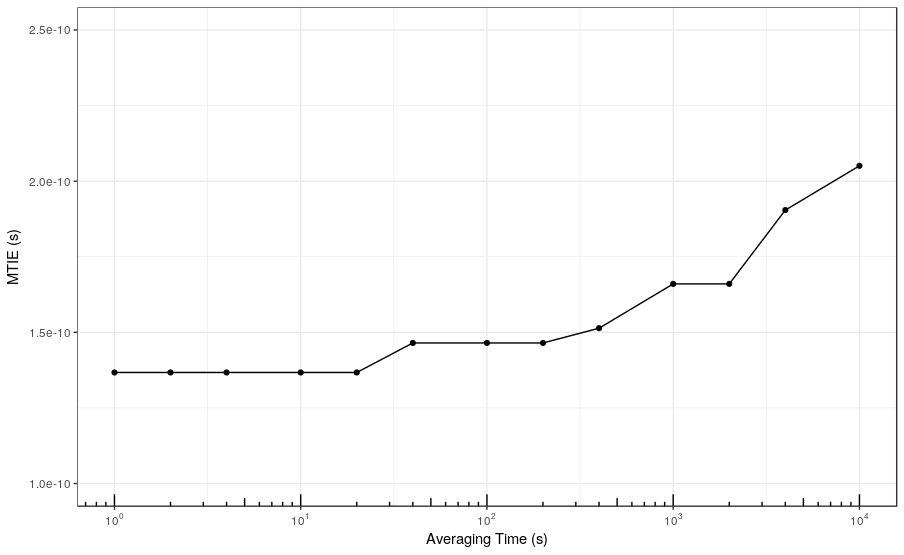
\includegraphics[width=0.9\linewidth]{img/MTIE_exp3}
	\caption[MTIE of the end-nodes in the scalability test.]{Maximum Time 
	Interval Error
	plot comparing the PPS signal from the end-nodes (WR-ZEN) to the Grand 
	Master of the network.}
	\label{fig:mtienet}
\end{figure}

\subsection{Fiber operational temperature influence on time accuracy}

One of the key aspects of the timing solution for the SKA facilities is the 
influence evaluation of the external elements in the timing performance. 
Synchronization signals are spread over hundred of nodes which are connected by 
long distance fiber links. Meteorological elements, such as wind or large 
 temperature changes, can alter propagation delays over the fiber 
links. The timing solution must compensate appropriately those effects in order 
to maintain the synchronization performance inside the limits required by the 
SKA's infrastructure.

On this contribution we've focused on the temperature change effect on the 
\textit{round-trip} (RTT) time and the PPS's performance. To evaluate that, we 
own a 
climate chamber in the laboratory and some fiber spools of tens of kilometers. 
We couldn't evaluate properly wind impact with our equipment, because of this, 
the experiments will only determine temperature effect on synchronization.

\ftgnote{Aquí un párrafo mencionando los efectos físicos sobre los haces de luz 
que viajan por la fibra al cambiar la temperatura. Índice de refracción. 
Aportar referencias!!!!}

Theoretically, WR, is able to dynamically calibrate the master to slave 
propagation delay from the total \textit{round-trip} time, \ftglnote{se 
necesita una ref aquí?} and therefore PPS offset shall maintain constant even 
when the propagation delay changes. The accurate estimation of the one-way 
propagation delay is achieved by the use of a constant value, $\alpha$, which 
express the ratio between propagation times with the two wavelengths used in 
the WR link. A complete explanation of the link model could be read in 
\cite{Wlostowski2011} and \cite{Daniluk2012}.

In the real world, $\alpha$ is temperature dependent, because of the change in 
the refraction index due to a temperature variation in the fiber. For small and 
mid-distance links, in laboratory conditions, $\alpha$ is nearly negligible and 
the current link model works very well. The WR network in SKA will be formed by 
long distance links exposed to external elements. In the concrete situation of 
the South Africa facilities, the chosen location was the Karoo region. 
\ftglnote{comprobar eso porque lo he sacado de Wikipedia} This region is a 
semi-desert area, very adequate to reduce human interferences in the high 
resolution data acquisition equipment, but with a inconvenient respec to the 
temperature point of view: desertic zones have a high difference between day 
and night temperatures.

We performed a series of experiments introducing a 50 km length fiber spool in 
a climate chamber. The RTT and the PPS's offset between master and slave were 
evaluated for a temperature range from 20 ºC to 50 ºC with 10 ºC steps. The 
average temperature difference between day and night in the Karoo region on 
each month is below 20 ºC, so the experiment covers comfortably the expected 
temperature operation conditions.

Our work hypothesis is that PPS's offset should keep constant for a varying 
RTT, in other words, the offset and the RTT do not present any kind of 
relationship between them. To prove this hypothesis, we have simulated the 
expected temperature conditions for a 50km fiber link using a climate chamber. 
Outside, in laboratory conditions, two WR-ZENs are connected using that fiber 
in a master-slave configuration. Then we've measured the offset of the PPS 
signal from slave to master with a timer (Keysight 53230A). The usual SFPs in 
WR deployments were not suitable for this experiment due to the long distance 
fiber link. We've used bidir SFPs from FiberStore with support up to 80 km 
distance links using 1550/1490 nm wavelengths. The setup schema is depicted in 
Figure ??. \ftglnote{hacer figura}

We had to perform the WR calibration procedure described in \cite{man:calib} to 
properly compensate the characteristic delays of the WR-ZEN board and the 
$\alpha$ constant of the used wavelengths. Once all the equipment was setup and 
calibrated, we started the thermal characterization of the link. To do that, we 
accomplished 4 independent experiments, where each one was related to one of 
the operation temperatures for the fiber spool. We started the measurement when 
the temperature of the system reached a stable point according to the targets. 

\begin{table*}\centering
	\ra{0.8}
	\begin{tabular}{@{} cccccc@{}}%\toprule
		& \multicolumn{2}{c}{\bfseries{RTT (ps)}} & &
		\multicolumn{2}{c}{\bfseries{PPS $offset_{SM}$ (ps)}} \\
		\cmidrule(l){2-3}  \cmidrule{5-6}
		\textbf{Spool temp (ºC)} & $\overline{x}$ & $s$ & & $\overline{x}$ 
		& $s$ \\ \midrule
	\small{20} & 479347020 & 365 & & 194 & 17 \\
	\small{30} & 478503719 & 50  & & 203 & 17 \\
	\small{40} & 478533492 & 807 & & 150 & 17 \\
	\small{50} & 478567050 & 399 & & 110 & 14 \\
	\bottomrule
	\end{tabular}
	\caption{Results of the thermal characterization for an operational fiber 
		temperature in range 20ºC to 50ºC with 10ºC steps.}
	\label{tab:temp}
\end{table*}

The most relevant results are included in Table \ref{tab:temp}: (i) the mean 
value of RTT and PPS offset samples, and (ii) their sample standard deviation. 
A total of 7200 samples (2 hours) have been used to compute the presented 
statistics. Round-trip time average for all the samples is 479347020 ps ($s=365 
ps$), and for the PPS offset we have an average of 194 ps ($s=17 ps$)
The correlation coefficient, expressed by the formula \ref{eq:r}, of the 
variables Offset (O) and RTT (R) is 0.08. This indicates a very weak linear 
relationship between both variables, which is just what we expected with our 
hypothesis.
Figure \ref{fig:ppsvsrtt} joins all the data from the experiments with 
different fiber temperature and makes visual that both variables are weakly 
related. Red line represents a fit linear model for the PPS offset given a RTT 
value. Line's slope is positive but with a very low increment. The reason for 
the deviation from 0 could be the use of a computed approximation of the real 
$\alpha$ value. 

\begin{equation}\label{eq:r}
r_{OR} = \frac{s_{OR}}{s_{O} s_{R}}
\end{equation}

The expected slave to master PPS offset related to distance and temperature of 
the fiber link is defined by the expression \ref{eq:offset}. We experimentally 
obtained that $k=0.13 ps$ \ftglnote{a javi: este k lo calculo de los valores 
medios experimentales, eso está bien? sería mejor con los del peor de los 
casos?}
\ftgnote{Comprobar el modelo haciendo una prueba con una fibra de 20km!!!!}

\begin{equation}\label{eq:offset}
	\hat{offset_{SM}} (T,d) = \frac {k ps} {T ºC \cdot d km}
\end{equation}

\begin{figure}
	\centering
	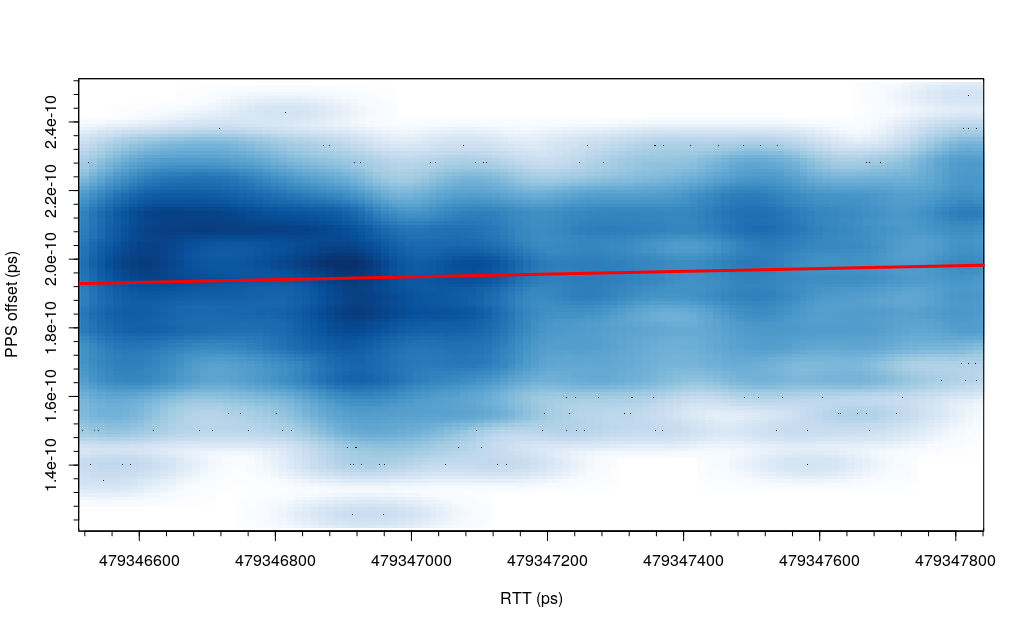
\includegraphics[width=1\linewidth]{img/ppsvsrtt}
	\caption[Evolution of the PPS offset and the RTT on multiple working 
	temperature for the fiber link]{Evolution of the PPS offset and the RTT on 
	multiple working temperature for the fiber link}
	\label{fig:ppsvsrtt}
\end{figure}
